\documentclass[conference]{IEEEtran}
\IEEEoverridecommandlockouts
% The preceding line is only needed to identify funding in the first footnote. If that is unneeded, please comment it out.
%Template version as of 6/27/2024

\makeatletter
\newcommand{\linebreakand}{%
  \end{@IEEEauthorhalign}
  \hfill\mbox{}\par
  \mbox{}\hfill\begin{@IEEEauthorhalign}
}
\makeatother

\usepackage{cite}
\usepackage{amsmath,amssymb,amsfonts}
\usepackage{algorithmic}
\usepackage{graphicx}
\usepackage{textcomp}
\usepackage{xcolor}
\usepackage{hyperref}
\usepackage{textcomp}
\usepackage{makecell} 
\usepackage{array}
\usepackage{tabularx}   % add this in preamble
\usepackage{amssymb}    % for \checkmark
\usepackage[greek,english]{babel}



\def\BibTeX{{\rm B\kern-.05em{\sc i\kern-.025em b}\kern-.08em
    T\kern-.1667em\lower.7ex\hbox{E}\kern-.125emX}}
\begin{document}

\title{Benchmarking Distributed SQL Query Execution with PrestoDB}

\author{    \IEEEauthorblockN{\textgreek{Εμμανουήλ Παντελάκης (03120853)}}
    \IEEEauthorblockA{\textit{School of Electrical and Computer Engineering} \\
        \textit{National Technical University of Athens}\\
        Athens, Greece \\
        TEAM ID: 02}
    \and
    \IEEEauthorblockN{\textgreek{Ιωάννης Δημουλάς (03120083)}}
    \IEEEauthorblockA{\textit{School of Electrical and Computer Engineering} \\
        \textit{National Technical University of Athens}\\
        Athens, Greece \\
        TEAM ID: 02}
    \linebreakand
    \IEEEauthorblockN{\textgreek{Ενρίκα Ηλιάνα Ματζόρι (03120143)}}
    \IEEEauthorblockA{\textit{School of Electrical and Computer Engineering} \\
        \textit{National Technical University of Athens}\\
        Athens, Greece \\
        TEAM ID: 02}
}

\maketitle

\begin{abstract}
    In today’s Age of Information, more and more aspects of our daily life are marked by an ever-growing volume of data. The need for efficient ways of processing and analyzing this “Big Data” is essential. This holds especially given that these large volumes of data are often distributed across multiple and extensive datasets managed by heterogeneous systems. In this context, PrestoDB, a distributed SQL query engine, has established itself as an invaluable tool for querying sizeable datasets spread across diverse data sources. This study investigates the performance of PrestoDB under various circumstances, including different data distribution plans, worker configurations, and query complexities. Our methodology includes finding a subset of the available TPC-DS benchmarks of varying complexity and iteratively executing them using different numbers of workers and data distributions. For the latter, we employ three distinct database management systems, those being PostgreSQL, MongoDB, and Apache Cassandra. We then compare execution times across configurations and derive insights into the behavior and optimization opportunities of each engine.\end{abstract}
\begin{IEEEkeywords}
    Big Data, PrestoDB, Distributed SQL Queries, Data Distribution, PostgreSQL, Apache Cassandra, MongoDB, TPC-DS Benchmark
\end{IEEEkeywords}

\section{Introduction}

The rapid growth of the Internet and significant advancements in digital technologies have dramatically increased the volume and variety of available data worldwide, giving birth to the concept of “Big Data”. Big data refers to massive, complex, and diverse datasets that grow exponentially over time and cannot be handled effectively by traditional data management systems. Analyzing big data can provide organizations and enterprises with useful insights, enabling them to make more informed business decisions \cite{b1,b2}. However, querying such vast amounts of data using traditional systems can be highly inefficient and costly, highlighting the need for new approaches to data management and distributed query processing. To address this challenge, in 2012, Facebook introduced PrestoDB.

PrestoDB is an open-source distributed SQL query engine designed to query large data sets across one or more heterogeneous data sources \cite{b3,b4}. Its ability to connect to a wide range of data sources---from traditional relational databases and modern NoSQL systems to data lakes---enables enterprises to analyze data without costly and time-consuming migrations, thereby maximizing the value of existing infrastructure.
Additionally, Presto can utilize multiple computational nodes to execute queries in parallel, leading to faster data processing and, thereby, accelerated decision-making.

This project aims to evaluate the performance of a Presto cluster by benchmarking it against a set of queries of varying complexity that operate on a large amount of data stored in a distributed manner across heterogeneous data sources. Specifically, the DBMSs included in this evaluation are the relational PostgreSQL, the columnar store Apache Cassandra, and the document-oriented MongoDB.

The dataset and queries used for the benchmarking are generated using the TPC-DS benchmark \cite{b5}. Queries span a range of operations, from simple SELECT statements to aggregations and complex multi-table joins, that act upon the entire dataset, while the dataset itself is several gigabytes in size, containing millions of records. The queries are executed using various distribution strategies across multiple workers, with execution times being recorded for each run. These measurements are then used to compare the efficiency of the different distributed methods and to evaluate the scaling performance of the Presto cluster.

This project is supported by a publicly available GitHub repository, which contains all scripts, configurations, and guidelines necessary to reproduce the PrestoDB cluster and the benchmarking experiments. The repository also includes the measurements obtained from the experiments and the graphs presented in this document.


\section{System Architecture and Software Description}\label{SystemArchitecture}

\subsection{Infrastructure Description}

For the purposes of our project, we were provided with two virtual machines by okeanos-knossos, a GRNET's IaaS cloud service for the Greek Research and Academic Community\cite{b6}.
The specifications of each virtual machine are as follows:

\begin{itemize}
    \item \textbf{CPU:} 8 virtual cores - Intel(R) Xeon(R) CPU E5-2650 v3
    \item \textbf{RAM:} 16 GB
    \item \textbf{Storage:} 60 GB (30 GB SSD plus an additional 30 GB of attached storage)
    \item \textbf{Operating System:} Ubuntu Server 24.04 LTS (upgraded from 16.04 LTS)
\end{itemize}

\subsection{PrestoDB}
Presto was originally developed by Facebook in 2012, aiming to address the performance restrictions of Apache Hive, the data warehouse Facebook used at the time. Apache Hive’s main issue was its inefficiency in handling large quantities of data, thereby creating the need for a better alternative. Facebook implemented PrestoDB, also known simply as Presto, an open-source distributed SQL query engine designed to query large data sets distributed over one or more heterogeneous data sources \cite{b3,b4}. Presto was designed with the following considerations: high performance, high scalability, adaptability, flexibility, and extensibility. It is capable of handling hundreds of resource-intensive queries concurrently and processing data from multiple and different data sources. Moreover, it can be configured to support a wide variety of use cases with diverse characteristics, accomplishing high performance due to its advanced query optimization techniques.

\subsubsection{Architecture Overview}

\begin{quote}
    ``A Presto cluster consists of a single coordinator node and one or more worker nodes. The coordinator is responsible for admitting, parsing, planning and optimizing queries as well as query orchestration. Worker nodes are responsible for query processing.'' \cite{b4}
\end{quote}

As shown in Figure~\ref{fig:presto-arch}, a client submits a query to the coordinator, as an ANSI SQL statement, via an HTTP request. The coordinator handles the incoming request by applying queue policies, parsing and analyzing the SQL statement, and generating an optimized distributed execution plan. This plan is then distributed to the worker nodes, which begin executing tasks. During this process, the coordinator specifies the number of splits, which represent addressable chunks of data in an external storage system. These splits are assigned to the appropriate tasks responsible for reading them. Worker nodes execute these tasks by retrieving data from external sources or by processing intermediate results produced by other workers. Since task execution on workers relies on cooperative multitasking, concurrent processing of multiple queries is achieved. In addition, execution is highly pipelined, which allows data to flow between tasks as soon as it becomes available.

\begin{figure}[htbp]
    \centering
    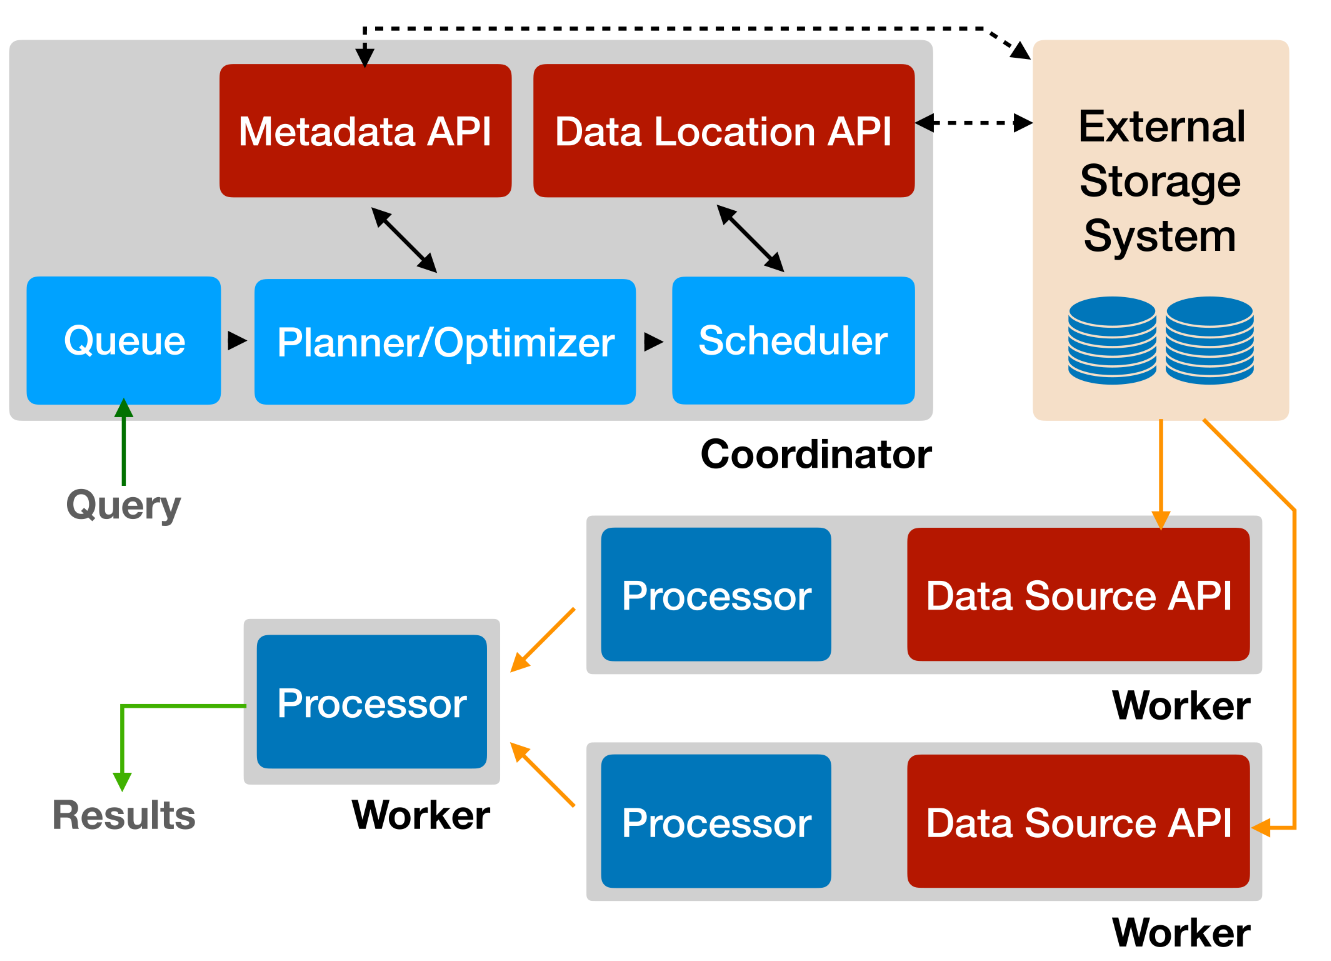
\includegraphics[width=\linewidth, keepaspectratio]{figures/presto-architecture.png}
    \caption{Presto Architecture \cite{b4}}
    \label{fig:presto-arch}
\end{figure}

Presto also offers a plugin interface that allows developers to extend it with custom data types, functions, access control implementations, event consumers, queuing policies, and configuration properties. Among these, the most crucial plugins are the connectors. The connectors enable Presto to connect with various external data stores through the Connector API, which is organized into four components: the Metadata, Data Location, Data Source, and Data Sink APIs. These APIs together support efficient connector implementations in a distributed execution environment.

\subsubsection{Node Types}

The \textit{coordinator} in a Presto cluster serves as the central node, the “brain” of the system, and is responsible for parsing SQL statements, generating query execution plans, handling the worker nodes and monitoring their activity, and orchestrating query execution across the cluster. It is also the endpoint through which clients submit their queries. Every Presto deployment requires one coordinator along with one or more worker nodes, although in a testing or development environment, a single Presto node can be configured to act as both the coordinator and a worker. The query execution process begins with the coordinator, which constructs a logical representation of the query, organizes it into multiple stages, and translates these stages into a set of interconnected tasks that are distributed among the workers.

Presto \textit{workers} are responsible for task execution and data processing. They retrieve data through connectors and exchange intermediate data with each other during query execution. The coordinator collects the data produced by the workers and delivers the final results to the client. When a worker node is launched, it registers itself in the cluster by advertising its presence to the coordinator’s discovery service, thereby becoming available for task assignment. Communication between workers and the coordinator, as well as among workers themselves, is performed through a REST API.


\subsubsection{Components}

A \textit{connector} in Presto is a plug-in that connects the Presto engine to an external catalog. It enables Presto to interact with a wide variety of data sources  for both reading and writing data, including relational databases, NoSQL databases, and filesystems. The connector’s role is to provide Presto with metadata, such as schemas, tables, and column definitions, and map the data from the external source into Presto’s data types. \cite{b7}

A \textit{catalog} represents a data source through its associated connector and contains one or more schemas. Each catalog is bound to a specific connector, and a query execution may operate across multiple catalogs. Catalogs are defined via properties files located in the configuration directory of each Presto node.

A \textit{schema} is used to organize tables within a catalog. Together, a catalog and schema define the set of tables that can be queried \cite{b3}. When accessing various data sources, a schema may either correspond to the same concept in the target database or, depending on the connector, organize the tables according to the data structure of the underlying source.

A \textit{table} in Presto, just like in a relational database, contains a set of rows, each arranged into named columns with associated data types. The way source data is represented as tables is determined by the connector.


\subsubsection{Query Execution Model}

Presto executes ANSI-compatible SQL statements by translating them into queries and devising a query plan that is then distributed across the worker nodes of the cluster.
\newline \indent In Presto, a \textit{statement} simply refers to the textual representation of a SQL query, which consists of clauses, expressions, and predicates.
A \textit{query} refers to the ensemble of components and configurations required to execute a statement, including stages, tasks, splits, connectors, and associated data sources, all working together to produce a result.

A \textit{query plan} outlines the sequence of steps required to retrieve and process data as specified in the SQL query \cite{b3}. It is structured as a tree of nodes, with each node representing an operator. Since SQL is declarative, multiple query plans can be devised to execute a given query, which may vary in performance. So, Presto relies on a query optimizer to select the most efficient one.
Presto’s \textit{query optimization} consists of two phases: logical and physical \cite{b3}. In the logical phase, the plan is refined by focusing exclusively on reducing the algorithmic complexity. Then, in the physical phase, the logically optimized plan is tailored for distributed execution by determining which Presto nodes will execute the query plan and the data exchange strategy between them.

When executing a query, Presto organizes the process into a hierarchy of \textit{stages} that form a tree-like structure. Each query has a root stage that collects and aggregates the results from other stages. While the stages define the distributed query plan, they are not executed directly on workers.
A \textit{stage} is executed as a collection of tasks distributed across the cluster’s worker nodes. Tasks serve as the core processing units within the architecture and operate on splits of data. The stages at the lowest level of a distributed query plan retrieve data through \textit{splits} provided by connectors, while intermediate stages consume data produced by preceding stages. During query scheduling, the Presto coordinator requests a list of all available splits for a table from the connector, tracks which tasks are processing those splits, and on which worker nodes they are running.
Essentially, the distributed query plan is first divided into stages, which are then further broken down into tasks that act upon or process these splits.  Each task has inputs and outputs and runs in parallel with other tasks, which in turn rely on multiple drivers for concurrent execution.
A \textit{driver} is the smallest unit of parallel execution in Presto, and it represents a pipeline of operator instances. Each driver consumes data, produces output by combining its operators, which is then aggregated by a task and forwarded to another task in another stage using an exchange client \cite{b3}.
An \textit{operator} is a processing unit that consumes data, performs a specific operation, such as filtering, projection, or joining, and emits results to be consumed by the next operator in the sequence.


\subsubsection{Query Optimization techniques}

When the Presto coordinator receives a new query from a client, it initiates the query optimizer in order to determine the most efficient execution strategy for the query. It does so by iteratively applying transformation rules until the optimal execution plan is found \cite{b4,b7}. Presto supports three query optimization strategies: predicate pushdown, cost-based optimization, and history-based optimization:

\textit{Predicate pushdown} \\
Predicate pushdown involves moving (``pushing down'') query predicates as close as possible to the data source. As a result, unnecessary data reads are minimized, thereby reducing I/O operations and network traffic, and improving query execution times. This strategy is particularly beneficial for queries involving joins with WHERE clauses, allowing Presto to filter unnecessary data before joining tables.\cite{b7}

\textit{Cost-based optimization (CBO)} \\
CBO is a strategy that evaluates query execution plans based on estimated computational costs. It relies on the table statistics, such as row counts and average column sizes, and leverages this information to determine the most effective join ordering strategy.\cite{b7}

\textit{History-based optimizations (HBO)} \\
HBO is a framework that records statistics from executed queries to reuse them for future queries with similar plans. To identify similar queries, each query plan is canonicalized to eliminate irrelevant differences, such as the naming of intermediate variables, and each plan node is hashed to a string value. Historical statistics associated with the same hash are then applied in HBO. These statistics are preferred over cost-based estimations, with the optimizer falling back to cost-based statistics when historical data is unavailable.\cite{b3}

Note that the connectors for Cassandra, PostgreSQL, and MongoDB do not support providing table statistics, which means that, in our case, Presto cannot utilize the CBO and HBO query optimization techniques.

\subsection{PostgreSQL}

PostgreSQL is an open-source object-relational database system or ORDBMS in abbreviation form \cite{b8}. It was the outcome adding the SQL language, in 1994, to the original POSTGRES package developed at the University of California, Berkeley. After more than three decades of its release, it has elevated itself as one of the most popular database management systems being used by large organizations; including Apple, Reddit, and Instagram \cite{b9}, largely because of its characteristics, briefly mentioned below:

As mentioned, PostgreSQL belongs to the ORDBMS family; thus, it adheres to the ACID properties. This stands for Atomicity, Consistency, Integrity, and Durability – a set of fundamental principles of relational database systems that ensures transaction integrity and data reliability \cite{b10, b11}.

At the same time, PostgreSQL is praised for its implementation of Multi-Version Concurrency Control (MVCC). This system allows concurrent transactions to access the same data without blocking one another. This feature renders PostgreSQL a very valuable tool, especially for maintaining high performance in environments with many simultaneous users \cite{b9}.

Flexibility and extensibility constitute another highly sought-after property. PostgreSQL is fairly versatile and enables developers to add new database functionality and packages without forking from the original project. Therefore, besides the native standard SQL data types, it has come to additionally support arrays, JSON/JSONB for semi-structured data, and even geospatial data \cite{b9,b12,b13}.

Finally, PostgreSQL uses vacuuming to manage storage overhead caused by multiple row versions, while also offering advanced query optimization through the usage of various indexing options; including B-Tree, GiST, GIN, and BRIN \cite{b9}.

This rich set of features, query capabilities, and transaction management, however, does not come without its drawbacks. The need for query optimization produces inefficiencies in big data storage and the suboptimal execution of certain types of transactions and join operations. The search for a solution to these problems has led to the emergence of the NoSQL database paradigm, to which both MongoDB and Apache Cassandra belong \cite{b14}.


\subsection{MongoDB}

MongoDB is an open-source NoSQL database developed by 10gen in 2007 in C++. It can be characterized as a Document Store – a type of NoSQL database. In this context, a document, basically, constitutes a record – a data structure composed of field value pairs. The type of documents used varies by vendor, but it is always defined by known standards, like XML and JSON. MongoDB, in particular, uses the latter \cite{b8, b14, b15}.

MongoDB, though non-relational, it yet implements many features common in relational databases, such as sorting, indexing, range queries and nested document queries \cite{b8}. Therefore, it inherits various advantages from both systems.

To begin with, MongoDB supports embedded data models, including documents and arrays. This, combined with the implementation of indexes for faster queries, leads to higher performance through the reduction of the I/O activity on the database system. At the same time, it provides rich query language capabilities for its users by handling both read and write operations, as well as data aggregation and text search. It ensures high availability by providing automatic failover and data redundancy across multiple servers, while lastly incorporating horizontal scalability through “sharding” – a process that distributes data across clusters of machines, thereby enhancing both performance and system capacity \cite{b15}.

The aforementioned set of features renders MongoDB a valuable compromise between efficient data storage and query execution. However, there are serious drawbacks that one must consider. Being a NoSQL database forces MongoDB to adhere to the CAP theorem. Theorised in 2000 by Brewer \cite{b16} and formally proved two years later by Gilbert and Lynch \cite{b17, b18}, it stands for Consistency, Availability, and Partition tolerance and it states that it is impossible for a distributed computing system to simultaneously provide all three guarantees. The choice of which feature to discard determines the nature of the system. MongoDB – among others – sacrifices consistency to get a scalable, simple, and high-performance database management system. Furthermore, since MongoDB is denormalized, it doesn’t need to follow a strict relational schema. While this allows for greater flexibility, it forces more schema-based design decisions on the app logic than the database itself \cite{b10, b15}.


\subsection{Apache Cassandra}

Cassandra is an open-source, highly scalable, distributed NoSQL database developed by the Apache Software Foundation and written in Java \cite{b14, b19}. Contrary to MongoDB, Cassandra belongs to another type of NoSQL database; that of Column stores. That is the type most similar to the traditional relational database model, where the column represents the unit of data identified by a key and a value. The main difference is that Cassandra retains much schema flexibility, being able to also handle semi-structured and unstructured data \cite{b14}.

However, perhaps the most highly sought-after feature Cassandra displays is that it is, in fact, designed to handle the storage of large amounts of data and the execution of millions of operations per day. It follows a peer-to-peer strategy, where data can be distributed all over the world, deployed across multiple nodes/data centres. When a node is added or removed, all data is automatically redistributed, allowing the failed node to be replaced with no downtime.
Durability is yet another strong point. Cassandra supports two different replication types: synchronous and asynchronous, with the user being able to opt for which one to use. A commit log is used to capture all writes and redundancies in order to ensure data durability.
Additionally, Cassandra makes use of indexing. Each node maintains all indexes of the tables it manages. It is, however, crucial to note that with larger data volumes and unique values, the amount of overhead created by the management of indexes is suboptimal \cite{b14}.



Cassandra’s flexible data model, no single point of failure, and linear scalability have rendered it ideal for video streaming services, like Netflix; but also for organizations with the need for big data management, including Apple, Facebook, IBM, Instagram, Rackspace, Twitter, Uber, Spotify, Cisco, eBay, etc. \cite{b20}.



\subsection{TPC-DS Benchmark}\label{tpcds}

The TPC-DS benchmark is a standard tool for measuring the performance of a decision support system. It achieves this by providing a set of SQL queries that can be executed on different systems to evaluate and compare their performance \cite{b5}.

This benchmark simulates a real-world business environment by employing large datasets and complex queries to assess how effectively a system can answer critical business questions, analyze trends, and manage data maintenance. To ensure applicability in real-world scenarios, TPC-DS defines 99 distinct SQL queries that cover a wide range of business analysis tasks \cite{b21}.

\subsubsection{Business Model}

TPC-DS models industries that manage, sell, and distribute a wide variety of products such as food, electronics, furniture, music, and toys. It adopts the business model of a large retail enterprise with multiple sales channels (physical stores, mail-order catalogs, and the internet), thus providing a realistic context.

The model not only provides tables for simulating sales and returns but also includes basic inventory management and promotional systems. The benchmark focuses on key business processes, which include:
\begin{itemize}
    \item Recording customer purchases and tracking returns across all sales channels.
    \item Modifying prices according to promotions.
    \item Maintaining warehouse inventory.
    \item Creating dynamic web pages.
    \item Maintaining customer profiles (Customer Relationship Management).
\end{itemize}

\subsubsection{Logical Database Design}

The logical database design of TPC-DS is centered around a snowflake schema, reflecting the complexity of a large retail enterprise. At its core are seven fact tables that capture the primary business processes of the benchmark:
\begin{itemize}
    \item \texttt{store\_sales} and \texttt{store\_returns}: purchases and returns from physical stores.
    \item \texttt{catalog\_sales} and \texttt{catalog\_returns}: purchases and returns from mail-order catalogs.
    \item \texttt{web\_sales} and \texttt{web\_returns}: purchases and returns through the online channel.
    \item \texttt{inventory}: modeling stock for the catalog and online channels.
\end{itemize}

In addition, the schema incorporates 17 dimension tables that provide descriptive context for the fact tables. These dimensions are shared across all sales channels and include details such as customer information, product attributes, time and date of transactions, and more.

Figures 2--8 illustrate the Entity-Relationship (ER) diagrams for each of the seven fact tables as provided by the TPC-DS Standard Specification \cite{b5}.

\begin{figure}[htbp]
    \centering
    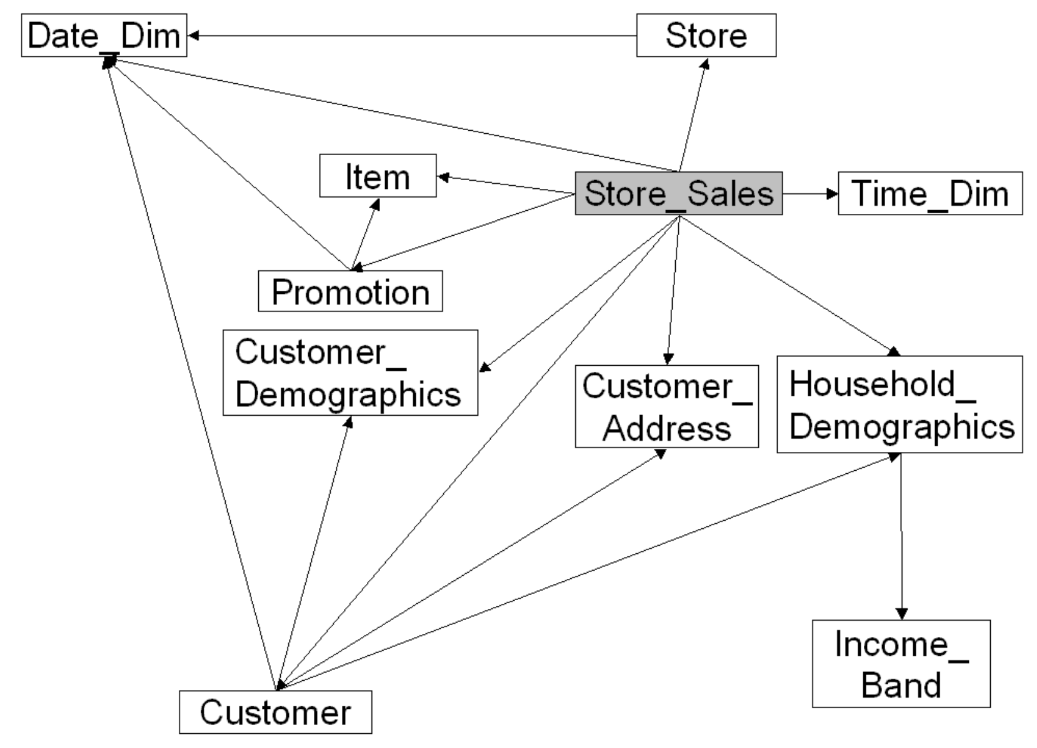
\includegraphics[width=\linewidth]{figures/fact_table_store_sales.png}
    \caption{ER Diagram of \texttt{store\_sales} fact table }
    \label{fig:store_sales}
\end{figure}

\begin{figure}[htbp]
    \centering
    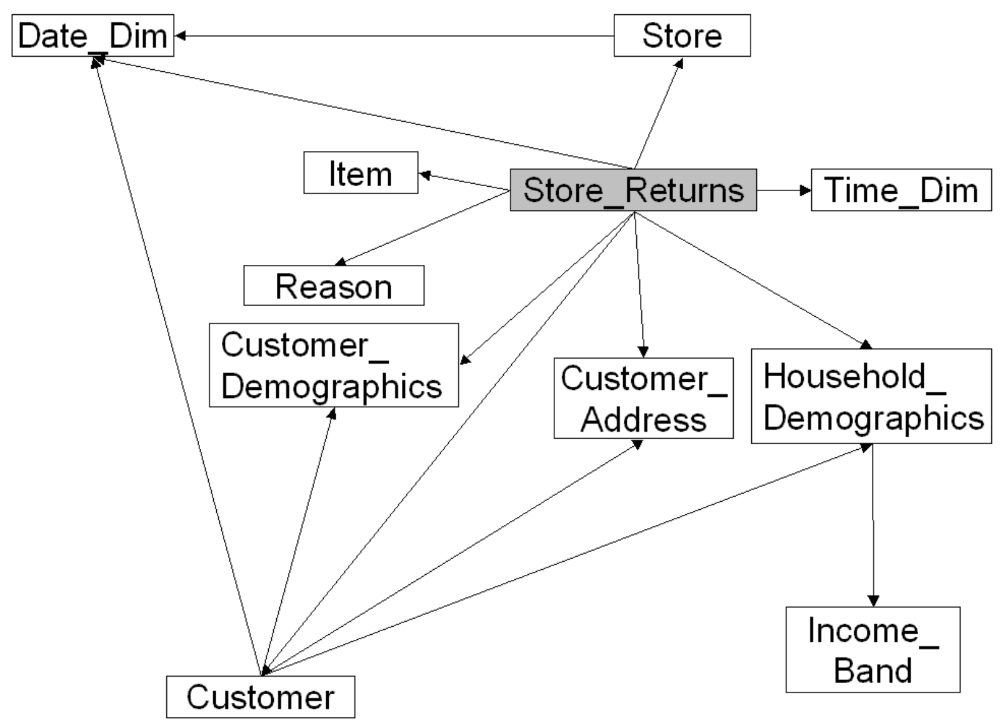
\includegraphics[width=\linewidth]{figures/fact_table_store_returns.png}
    \caption{ER Diagram of \texttt{store\_returns} fact table }
    \label{fig:store_returns}
\end{figure}

\begin{figure}[htbp]
    \centering
    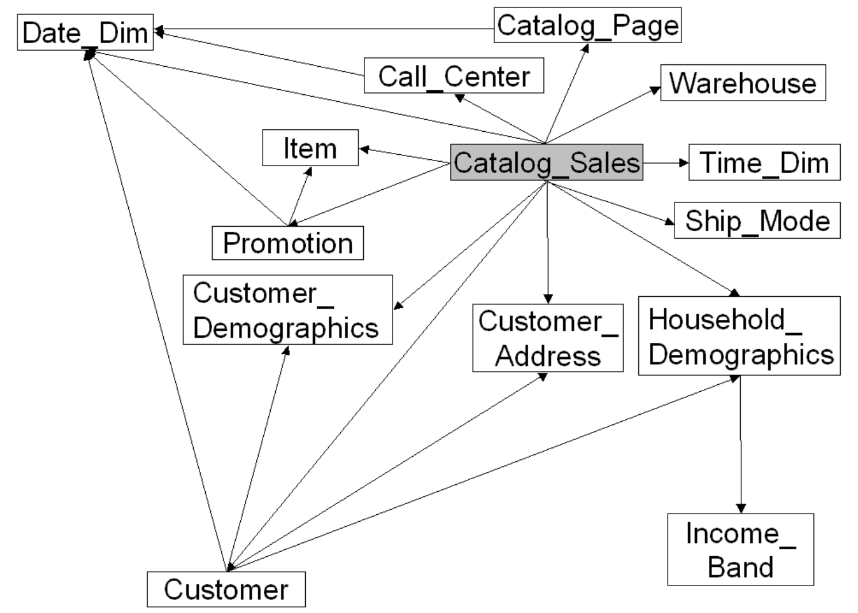
\includegraphics[width=\linewidth]{figures/fact_table_catalog_sales.png}
    \caption{ER Diagram of \texttt{catalog\_sales} fact table }
    \label{fig:catalog_sales}
\end{figure}

\begin{figure}[htbp]
    \centering
    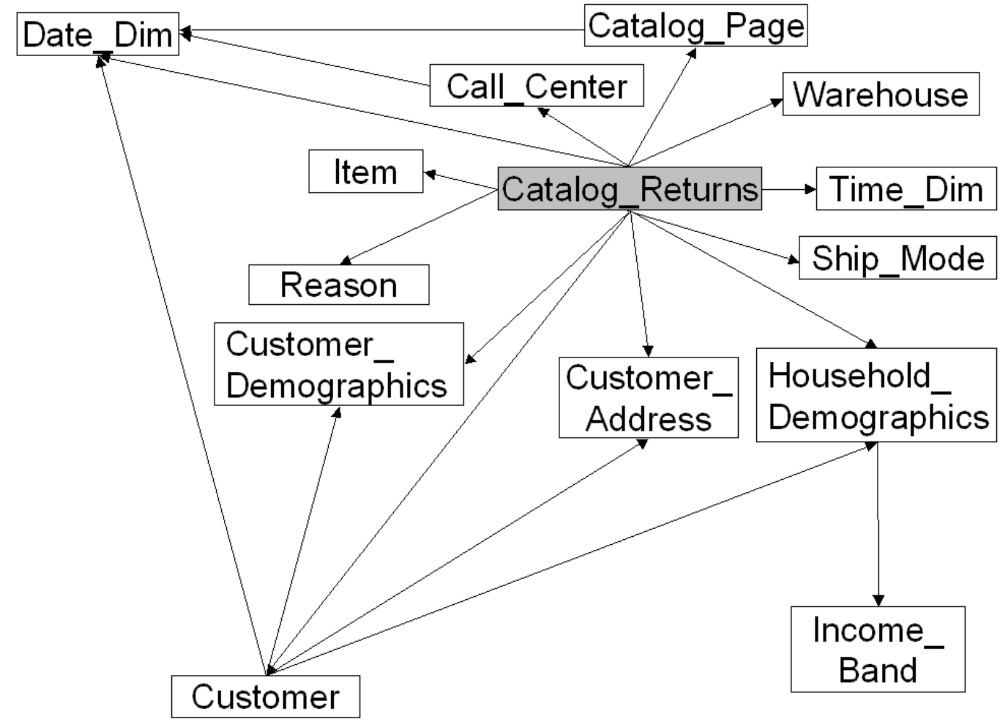
\includegraphics[width=\linewidth]{figures/fact_table_catalog_returns.png}
    \caption{ER Diagram of \texttt{catalog\_returns} fact table }
    \label{fig:catalog_returns}
\end{figure}

\begin{figure}[htbp]
    \centering
    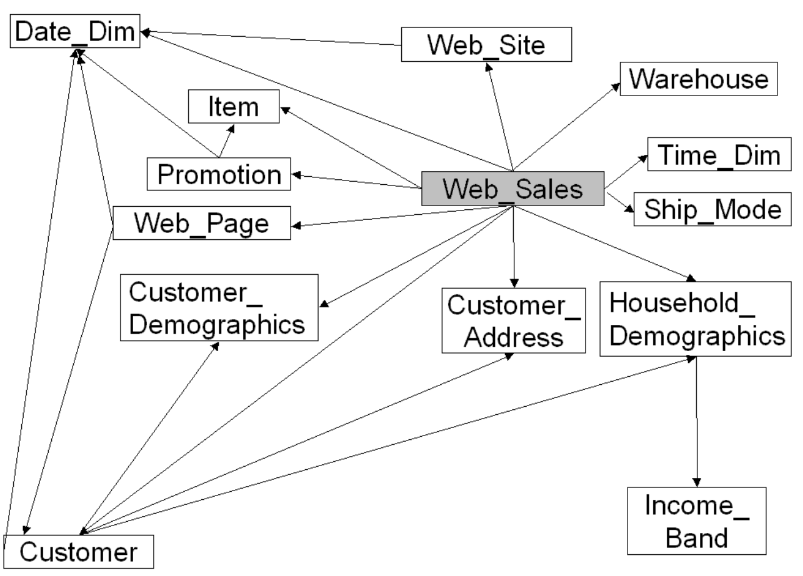
\includegraphics[width=\linewidth]{figures/fact_table_web_sales.png}
    \caption{ER Diagram of \texttt{web\_sales} fact table }
    \label{fig:web_sales}
\end{figure}

\begin{figure}[htbp]
    \centering
    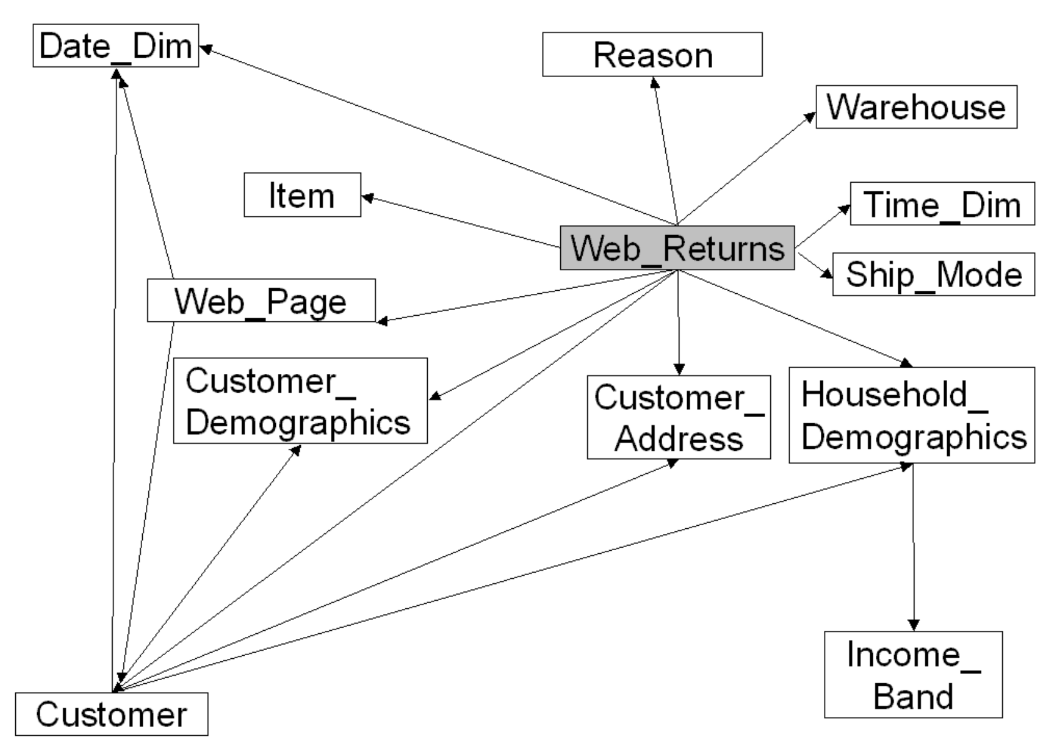
\includegraphics[width=\linewidth]{figures/fact_table_web_returns.png}
    \caption{ER Diagram of \texttt{web\_returns} fact table }
    \label{fig:web_returns}
\end{figure}

\begin{figure}[htbp]
    \centering
    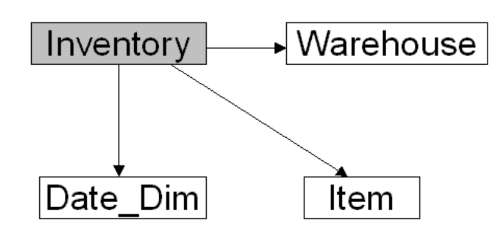
\includegraphics[width=\linewidth]{figures/fact_table_inventory.png}
    \caption{ER Diagram of \texttt{inventory} fact table }
    \label{fig:inventory}
\end{figure}

\subsubsection{Query Classes}

The TPC-DS benchmark provides a set of queries that we used to design the appropriate data distribution strategy. These queries can be classified into four main categories, based on the type of user and the information they are intended to retrieve from the decision support system:

\begin{itemize}
    \item \textbf{Reporting queries:} Queries that answer pre-defined questions, often with minor variations such as date range or location.
    \item \textbf{Ad hoc queries:} Queries that dynamically answer immediate and specific business questions, in contrast to the pre-planned nature of reporting queries.
    \item \textbf{Iterative OLAP queries:} Queries aimed at exploring and analyzing data to discover new relationships and trends.
    \item \textbf{Data mining queries:} Queries that sift through large amounts of data to uncover relationships and predict future trends, typically involving large joins and aggregations. \cite{b5}
\end{itemize}

\section{Source Code}\label{source_code}

All configuration files, scripts, and guidelines required to set up the Presto cluster are available in a dedicated GitHub repository. This repository serves as a complete reference for reproducing the cluster environment, including the installation and configuration of PrestoDB, instructions for installing the database management systems, generating the TPC-DS benchmark data, and importing it into the database systems. It also includes the benchmarking results and the graphs presented in this document.

The repository can be accessed at the following link:

\begin{center}
    \href{https://github.com/mpantelakis/ntua-information-systems}{GitHub Repository}
\end{center}


\section{Installation and Configuration}

\subsection{PrestoDB Cluster Setup}

Due to the limited available resources, we cannot create a Presto cluster with multiple workers, where each functions as an independent computing node. Therefore, to make full use of the available resources, the workers must be treated as processes on the same machine, sharing its resources in a way that simulates independent compute nodes (where feasible). To this end, we have distributed the 16 total CPU cores of the two machines between the coordinator and three workers. Using the Linux \texttt{taskset} command, we have assigned each process to a specific 4-core set. The coordinator and first worker share the first machine's cores, and the other two workers share the second machine's cores. Additionally, we have limited the total available memory for each node to 4 GB through the JVM configuration file.

Regarding the database systems, due to the high memory requirements of the Cassandra system, we have chosen to install it alone on the first machine, while MongoDB and PostgreSQL are installed on the second machine. Figure~\ref{fig:cluster_topology} illustrates the overall topology of the cluster.

\begin{figure}[htbp]
    \centering
    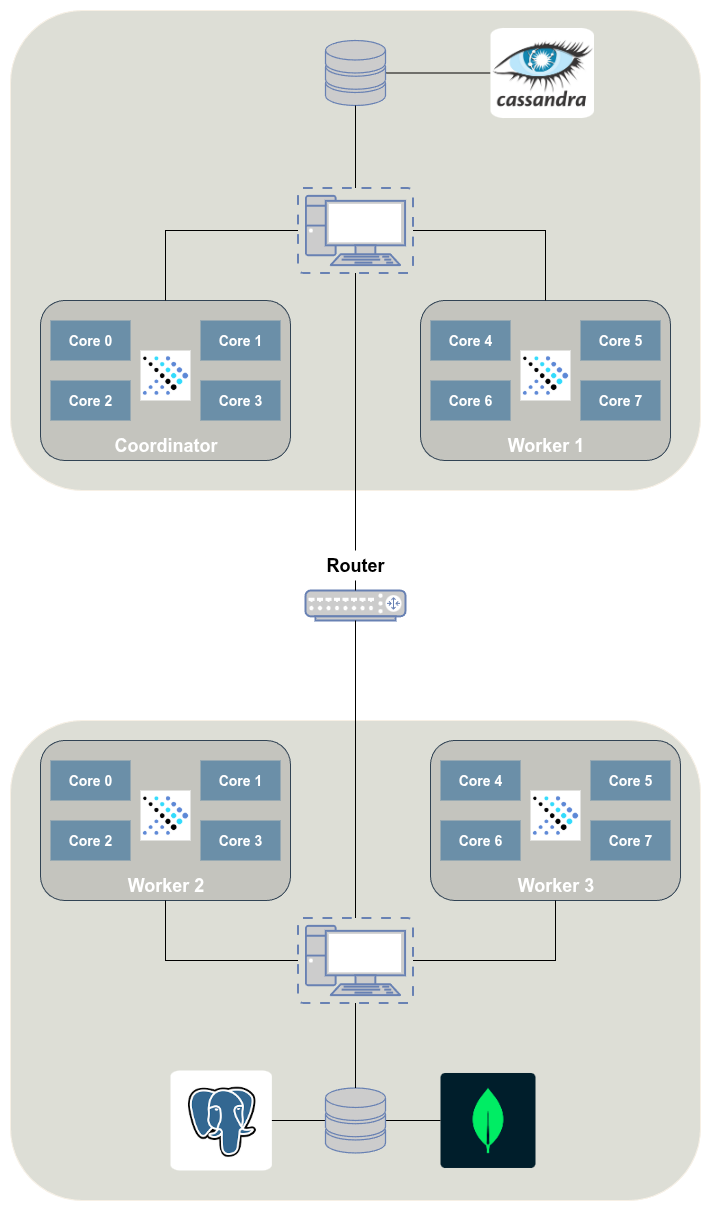
\includegraphics[width=\linewidth]{figures/cluster_topology.png}
    \caption{PrestoDB Cluster Topology }
    \label{fig:cluster_topology}
\end{figure}

It is clear that the network connectivity between the machines is not ideal, as they do not belong to the same subnet. Consequently, data transfers between the nodes are subject to potential delays, making the cluster's performance highly dependent on the available network bandwidth and latency.

\subsection{PrestoDB Nodes Configuration}

Each Presto node resides within its own Presto installation folder. Within this folder, it is necessary to define the \texttt{etc} directory, which contains the following configuration files:

\begin{itemize}
    \item \textbf{Node Properties} (\texttt{node.properties}): Specifies environment-specific settings for each Presto node, such as the node ID.
    \item \textbf{JVM Config} (\texttt{jvm.config}): Contains command-line options for the Java Virtual Machine running the Presto node.
    \item \textbf{Config Properties} (\texttt{config.properties}): Defines Presto server configurations, including coordinator/worker settings and query-related parameters.

    \item \textbf{Log Properties} (\texttt{log.properties}): Configures logging for the Presto node, including log levels and format.
\end{itemize}


Inside the \texttt{etc} directory, there must also be a \texttt{catalog} directory containing all the connectors, one for each database system (e.g., \texttt{cassandra.properties}, \texttt{mongodb.properties}, \texttt{postgresql.properties}).

Finally, within the installation folder, it is necessary to create the \texttt{data} directory, which will store all log files.


\subsection{TPC-DS Benchmark Data \& Queries Generation}

The TPC-DS Benchmark Suite provides the capability to generate data through the tool \texttt{dsdgen}. It produces data by taking as main parameters the scale factor, i.e., the total size of the data in GB to be generated, and the output directory. Below is an example execution of \texttt{dsdgen} for generating data with a total size of 1GB:

\begin{verbatim}
dsdgen -scale 1 -dir /home/user/tpcds-data
\end{verbatim}

To determine the total data size to be generated, we had to account for the limited storage available, which was further constrained by PostgreSQL and MongoDB sharing the same storage device. As mentioned in Section~\ref{no_dist}, the base benchmarks required loading the entire dataset into each database system, which created an additional limitation. After testing, we selected a total data size of 8 GB. It is worth noting that, although the overall dataset size was 8.6 GB, the actual storage occupied by each system varied. Specifically, the observed data sizes in each system were:

\begin{itemize}
    \item Cassandra: 5.9 GB
    \item MongoDB: 10.58 GB
    \item PostgreSQL: 17 GB
\end{itemize}


In addition to data generation, the TPC-DS Benchmark Suite also offers 99 query templates for benchmarking purposes. These templates can be converted into executable SQL queries using the tool \texttt{dqgen}. In Section~\ref{query_selection}, we describe the process of selecting some of these queries to use in our benchmarks.


\subsection{Data Population of Database Systems}

To load the generated data into the three database systems, we created two Bash scripts,
one for Cassandra and one for PostgreSQL, and a Python script for MongoDB.

For Cassandra, we used the native client \texttt{cqlsh} with the \texttt{COPY} command.
For PostgreSQL, we used its native client as well.

However, for MongoDB we did not use the official data import tool, \texttt{mongoimport},
since it does not support the ``\texttt{|}'' delimiter (used by TPC-DS when generating data).
Instead, we developed a Python script using the \texttt{pymongo} library.

All three scripts are available in the GitHub repository referenced in Section~\ref{source_code}.

\section{Benchmark Query Selection and Classification}\label{query_selection}

We selected a subset of 28 out of the 99 total queries. The selection was done carefully, checking that all fact tables were used and having both a structural and a logical variety in each single query. The queries were then organized into two main dimensions: their complexity and the number of fact tables accessed within the query.

Within these dimensions, we created five groups in total: three focused on complexity, and two related to the number of fact tables used. Specifically:

\begin{enumerate}
    \item \textbf{Complexity Classification:} The 28 queries were split into three categories based on their structural complexity:
          \begin{itemize}
              \item \textit{Simple Complexity:} The queries in this category are characterized by basic operations along with simple aggregation functions, without the use of advanced subqueries or complex Common Table Expressions (CTEs).
              \item \textit{Medium Complexity:} The queries in this category are characterized by a more advanced structure, with numerous aggregations and complex logic through the use of nested subqueries and CTEs.
              \item \textit{High Complexity:} The queries in this category are characterized by a high degree of complexity. They feature multiple CTEs, extensive use of nested subqueries, and complex join operations.
          \end{itemize}
    \item \textbf{Fact Table Access Classification:} The 28 queries were split into two groups based on the number of fact tables they interact with:
          \begin{itemize}
              \item \textit{Single Fact Table:} The queries in this category access only one fact table.
              \item \textit{Multiple Fact Table:} The queries in this category access multiple fact tables.
          \end{itemize}
\end{enumerate}

So, the total of 5 groups allowed us to gain a whole view of the 3 DBMS we had and how each change affected the whole system. In this way, we can design the appropriate data distribution strategy to maximize the system’s performance.

The selected queries and their categorization into respective groups are shown in Table~\ref{tab:query_groups}.

\begin{table}[htbp]
    \centering
    \renewcommand{\arraystretch}{1.3}
    \caption{Categorization of the selected TPC-DS queries}
    \begin{tabular}{|>{\centering\arraybackslash}c|>{\centering\arraybackslash}m{6cm}|} % use m{6cm} for vertical centering
        \hline
        \textbf{Group}               & \textbf{Queries}                                                         \\
        \hline
        \textbf{Simple Complexity}   & 1, 2, 7, 14, 15, 16, 20, 23, 32                                          \\
        \hline
        \textbf{Medium Complexity}   & 5, 8, 12, 13, 17, 21, 22, 24, 39, 94                                     \\
        \hline
        \textbf{High Complexity}     & 3, 4, 6, 9, 10, 30, 37, 48, 49                                           \\
        \hline
        \textbf{Single Fact Table}   & 1, 2, 4, 5, 7, 8, 12, 13, 14, 15, 16, 21, 23, 24, 30, 32, 37, 39, 49, 94 \\
        \hline
        \textbf{Multiple Fact Table} & 3, 6, 9, 10, 17, 20, 22, 48                                              \\
        \hline
    \end{tabular}
    \label{tab:query_groups}
\end{table}

Note that, in order to implement an effective data distribution strategy, we carefully selected a set of queries from all four categories described in Section~\ref{tpcds} to ensure that the system’s performance would be both optimal and representative across the full range of real-world business intelligence tasks \cite{b5}.

\section{Data Distribution Strategies and Results Analysis}

With the selection of a diverse set of queries, showcasing varying degrees of complexity and needs, completed, the next step is to devise different strategies to distribute our data into the three heterogeneous database management systems, as well as different worker configurations. The strategies must be selected in a way that gives us useful insights into the distributed execution engine’s behavior. Our ultimate goal is to optimize query performance. In this section, we describe, analytically, the plans we formulated to this end, and the corresponding results.

\subsection{No Data Distribution Applied}\label{no_dist}

For our first experiment, we actually measured the performance of every database management system independently from one another, without implementing any form of data distribution. This decision was made in order to test in practice their strengths and weaknesses, as they were discussed in Section~\ref{SystemArchitecture}, , to view how they handle different query operations and needs, and, in general, to establish a baseline understanding of each DBMS. To this end, we ran – with a single worker at a time – each group’s queries five times for every DBMS, and we recorded the execution time. Afterwards, we calculated the arithmetic means of the execution times per query for every group and plotted them. The results of this process are shown in Figure~\ref{fig:no_dist_applied}.

\begin{figure}[htbp]
    \centering
    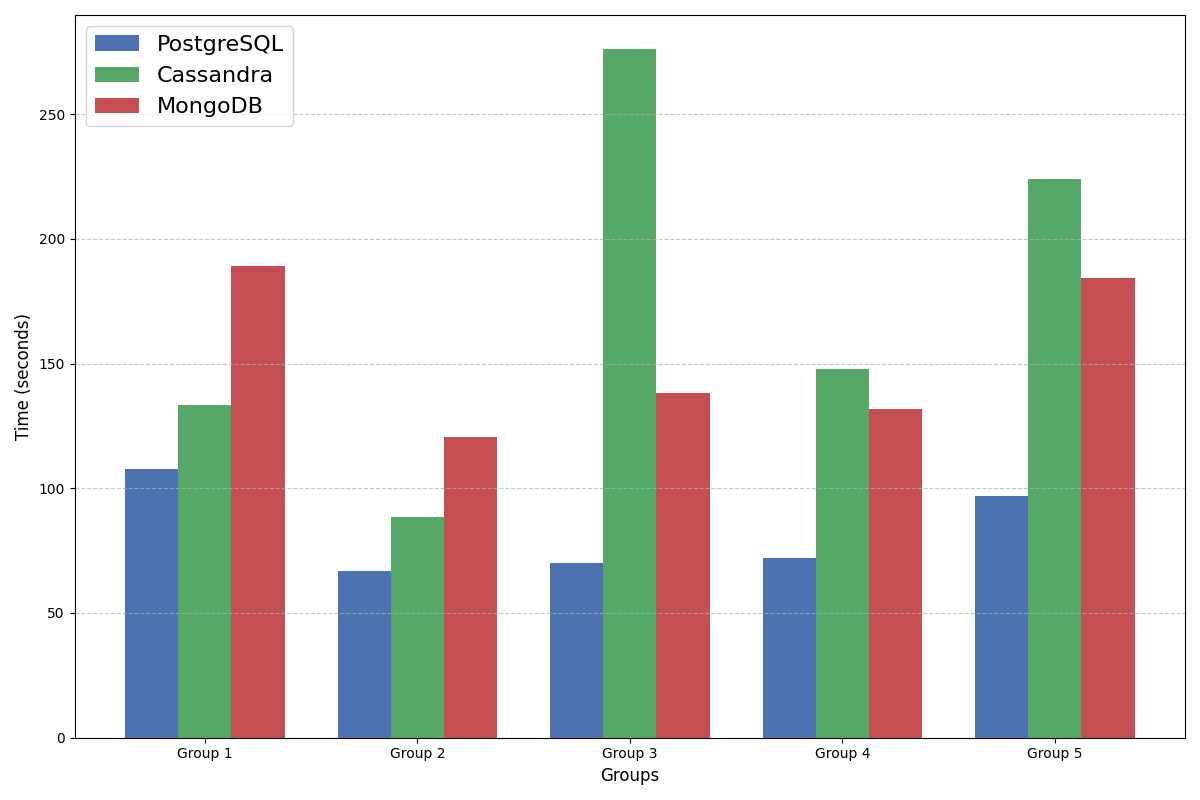
\includegraphics[width=\linewidth]{figures/no_dist_applied.png}
    \caption{Average Execution Time by Group and Database System - No Distribution Applied}
    \label{fig:no_dist_applied}
\end{figure}

The first thing to notice is that PostgreSQL achieves steadily lower query execution times relative to the other two database systems across all five groups. This confirms the theoretical superiority of object-relational database systems regarding query execution performance. However, it must be reminded that despite its high operation efficiency, PostgreSQL lacks in data storage efficiency.

Regarding the two NoSQL databases – MongoDB and Cassandra – the results are less straightforward. As the complexity of the queries remains relatively low for the first two groups, Cassandra achieves lower execution times than MongoDB; it is around 40\% quicker. However, for group 3, we have a completely different image. Cassandra seems incapable of handling the high complexity and large computational resources needed for the queries involved. It lacks efficient support for ad-hoc or multi-dimensional queries. On the contrary, MongoDB gains heavily from the way it organizes its data and its indexing strategies, enabling it to handle a broader range of query patterns more gracefully. This trend continues with both groups 4 and 5.

To conclude the results from the first experiment with no data distribution, PostgreSQL appears to be the most reliable across all query groups. Cassandra and MongoDB exhibit mixed results; however, the performance collapse of the former for queries of higher complexity will be taken into consideration when moving to the next data distribution strategies.

\subsection{Fact Table Size \& ER Based Distribution}

We based the first method of distributing the data across the three systems solely on the size of the fact tables and the previous results regarding the overall performance of each system. Initially, we sorted the fact tables in descending size order, as shown in Table~\ref{tab:fact_table_sizes}, based on the size of the data files generated by TPC-DS for each table.

\begin{table}[htbp]
    \centering
    \renewcommand{\arraystretch}{1.2}
    \caption{Sizes of TPC-DS fact tables}
    \begin{tabular}{|l|c|}
        \hline
        \textbf{Fact Table} & \textbf{Size} \\
        \hline
        store\_sales        & 3.0 GB        \\
        catalog\_sales      & 2.3 GB        \\
        inventory           & 1.6 GB        \\
        web\_sales          & 1.2 GB        \\
        store\_returns      & 256 MB        \\
        catalog\_returns    & 168 MB        \\
        web\_returns        & 78 MB         \\
        \hline
    \end{tabular}
    \label{tab:fact_table_sizes}
\end{table}


The goal was to assign an appropriate data volume of the fact tables to each system in proportion to its demonstrated performance. PostgreSQL, which demonstrated the best performance, was assigned the largest data volume (store\_sales and catalog\_sales), while MongoDB and Cassandra were assigned smaller data volumes (inventory, web\_sales and store\_returns, catalog\_returns, web\_returns, respectively). Cassandra naturally handled the smallest volume. The dimension tables are loaded in each system according to the ER of the fact tables they host. In other words, the dimension tables are duplicated or triplicated within the cluster.
The overall distribution of tables across the three systems is summarized in Table~\ref{tab:table_distribution_1}, while the corresponding benchmarking results are shown in Figure~\ref{fig:dist_method_1}.

\begin{figure}[htbp]
    \centering
    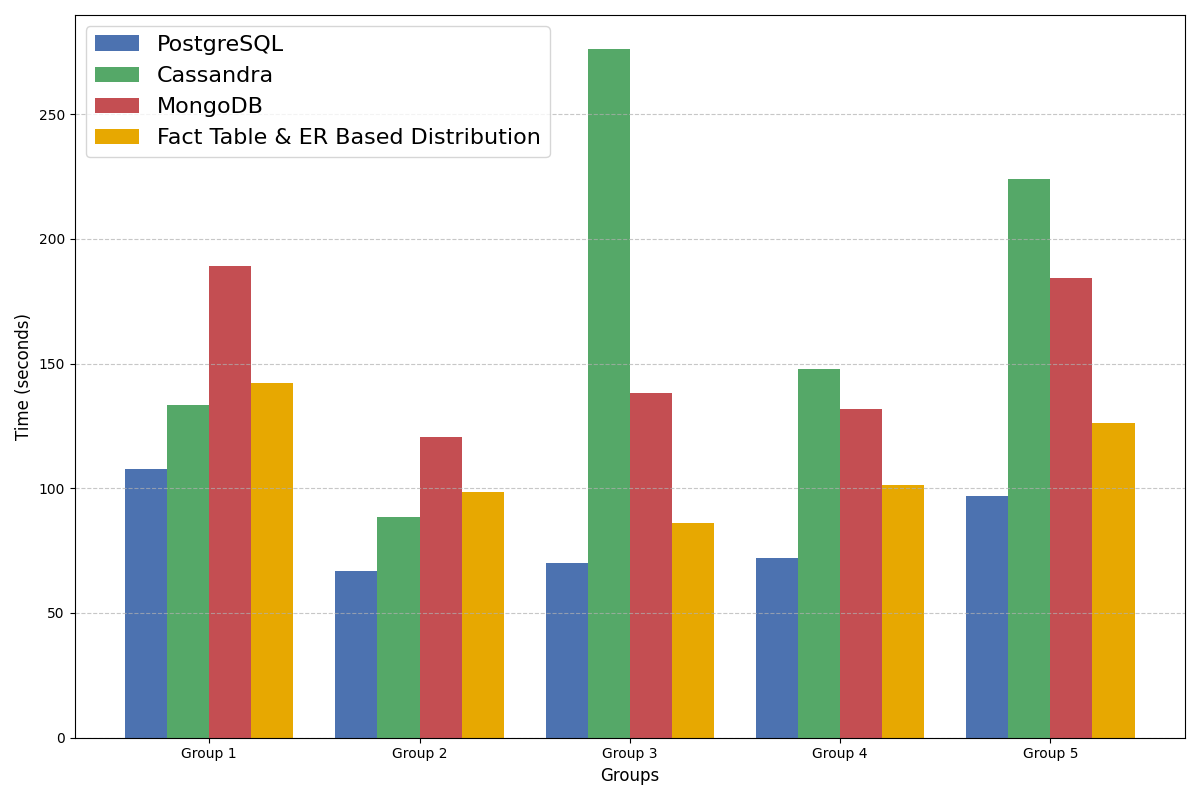
\includegraphics[width=\linewidth]{figures/dist_method_1.png}
    \caption{Average Execution Time by Group - Fact Tables \& ER Based Distribution Method}
    \label{fig:dist_method_1}
\end{figure}


\begin{table}[htbp]
    \centering
    \renewcommand{\arraystretch}{1.2}
    \caption{Fact Table Size \& ER-Based Distribution Method - Data Distribution}
    \resizebox{\linewidth}{!}{%
        \begin{tabular}{|l|c|c|c|}
            \hline
            \textbf{Table}          & \textbf{PostgreSQL} & \textbf{MongoDB} & \textbf{Cassandra} \\
            \hline
            call\_center            & \checkmark          &                  & \checkmark         \\
            catalog\_page           & \checkmark          &                  & \checkmark         \\
            catalog\_returns        &                     &                  & \checkmark         \\
            catalog\_sales          & \checkmark          &                  &                    \\
            customer                & \checkmark          & \checkmark       & \checkmark         \\
            customer\_address       & \checkmark          & \checkmark       & \checkmark         \\
            customer\_demographics  & \checkmark          & \checkmark       & \checkmark         \\
            date\_dim               & \checkmark          & \checkmark       & \checkmark         \\
            household\_demographics & \checkmark          & \checkmark       & \checkmark         \\
            income\_band            & \checkmark          & \checkmark       & \checkmark         \\
            inventory               &                     & \checkmark       &                    \\
            item                    & \checkmark          & \checkmark       & \checkmark         \\
            promotion               & \checkmark          & \checkmark       &                    \\
            reason                  & \checkmark          &                  & \checkmark         \\
            ship\_mode              & \checkmark          & \checkmark       & \checkmark         \\
            store                   & \checkmark          &                  & \checkmark         \\
            store\_returns          &                     &                  & \checkmark         \\
            store\_sales            & \checkmark          &                  &                    \\
            time\_dim               & \checkmark          & \checkmark       & \checkmark         \\
            warehouse               & \checkmark          & \checkmark       & \checkmark         \\
            web\_page               & \checkmark          & \checkmark       & \checkmark         \\
            web\_returns            &                     &                  & \checkmark         \\
            web\_sales              &                     & \checkmark       &                    \\
            web\_site               & \checkmark          & \checkmark       &                    \\
            \hline
        \end{tabular}%
    }
    \label{tab:table_distribution_1}
\end{table}

This first attempt at distributing the data achieves execution times between those of PostgreSQL and the NoSQL systems. It does not match PostgreSQL’s single-node performance, but it provides a good balance and demonstrates that distributing based on fact table size \& ER relationships reduces overhead compared to MongoDB and Cassandra individually. The improvement comes mainly from balancing the workload proportionally to each system’s strengths. PostgreSQL was assigned the heaviest fact tables, thereby preventing Cassandra or MongoDB from being overloaded with data volumes that they cannot process effectively. The biggest improvement compared to not applying any distribution is visible in Group 3 (high-complexity queries), where it clearly outperforms MongoDB and Cassandra by a significant margin, although still behind PostgreSQL. More specifically, our first distribution method outperformed Cassandra in Groups 3, 4, and 5 by 220\%, 45\% and 77\% respectively, while it outperformed MongoDB in all groups, showcasing an improvement in performance ranging from 23\% to 60\%.


\subsection{Logical Fact Table Pair Distribution}

Designing our second distribution strategy, we kept the same basic principle as before: each fact table was grouped with its associated dimension tables, as indicated by the ER diagrams. However, now we also took advantage of the logical relationships between fact tables. Specifically, we noticed that certain fact tables form pairs based on their meaning. A simple example is the pair store\_sales and store\_returns. The logical connection between these tables often makes them appear together in queries. This thought was confirmed through an observation of our query set, which showed that a large proportion followed this pattern. Based on this insight, we adjusted the strategy so that each of these logical pairs was placed in the same DBMS, along with their corresponding dimension tables.

The exact distribution selected in this experiment is shown in Table~\ref{tab:table_distribution_2}.
\begin{table}[htbp]
    \centering
    \renewcommand{\arraystretch}{1.2}
    \caption{Logical Fact Table Pair Distribution Method - Data Distribution}
    \resizebox{\linewidth}{!}{%
        \begin{tabular}{|c|c|c|c|}
            \hline
            Table                   & PostgreSQL & MongoDB    & Cassandra  \\
            \hline
            call\_center            & \checkmark & \          & \          \\
            catalog\_page           & \checkmark & \          & \          \\
            catalog\_returns        & \checkmark & \          & \          \\
            catalog\_sales          & \checkmark & \          & \          \\
            customer                & \checkmark & \checkmark & \          \\
            customer\_address       & \checkmark & \checkmark & \          \\
            customer\_demographics  & \checkmark & \checkmark & \          \\
            date\_dim               & \checkmark & \checkmark & \checkmark \\
            household\_demographics & \checkmark & \checkmark & \          \\
            income\_band            & \checkmark & \checkmark & \          \\
            inventory               & \          & \          & \checkmark \\
            item                    & \checkmark & \checkmark & \checkmark \\
            promotion               & \checkmark & \checkmark & \          \\
            reason                  & \checkmark & \checkmark & \          \\
            ship\_mode              & \checkmark & \checkmark & \          \\
            store                   & \checkmark & \          & \          \\
            store\_returns          & \checkmark & \          & \          \\
            store\_sales            & \checkmark & \          & \          \\
            time\_dim               & \checkmark & \checkmark & \          \\
            warehouse               & \checkmark & \checkmark & \checkmark \\
            web\_page               & \          & \checkmark & \          \\
            web\_returns            & \          & \checkmark & \          \\
            web\_sales              & \          & \checkmark & \          \\
            web\_site               & \          & \checkmark & \          \\
            \hline
        \end{tabular}
    }
    \label{tab:table_distribution_2}
\end{table}


Figure~\ref{fig:dist_method_2} illustrates the performance improvement of this distribution method over the previous one that ranges from 15.18\% to 28.9\% across different query groups. Notably, the new strategy achieved execution times close to those of a single-node PostgreSQL system, highlighting a significant gain in efficiency.

\begin{figure}[htbp]
    \centering
    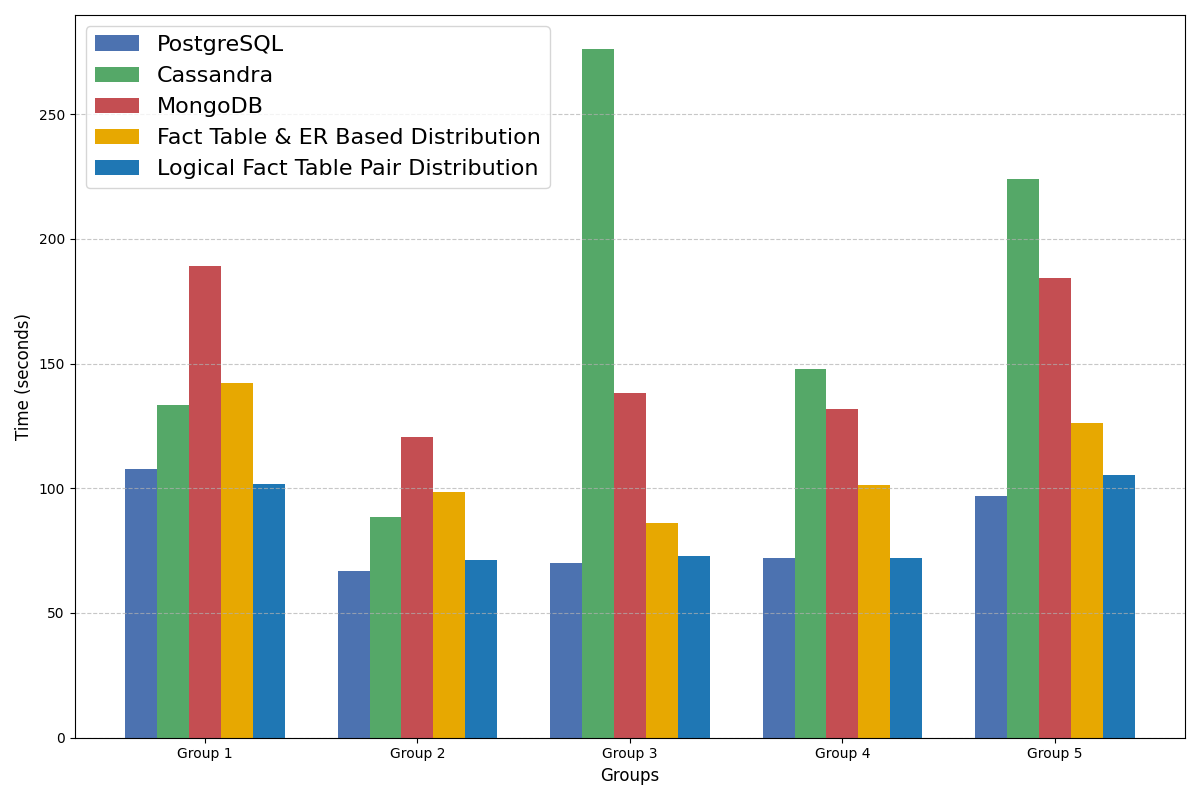
\includegraphics[width=\linewidth]{figures/dist_method_2.png}
    \caption{Average Execution Time by Group - Logical Fact Table Pair Distribution Method}
    \label{fig:dist_method_2}
\end{figure}

The distribution choice of storing logically related fact tables together helped reduce the inter-database communication required for executing queries that involve both fact tables of a pair. By keeping sales-returns fact tables couples within the same DBMS, latency and overhead were significantly reduced leading to a more efficient query execution, with performance approaching that of a non-distributed database.


\subsection{Frequency-Based Dimension Table Distribution}

Our third distribution strategy was developed to improve the previous approach, which gave us the best results so far. In the two previous strategies, the dimension tables were placed together with their associated fact tables based on the ER diagram. However, this involved the repetition of dimension tables across the system. This redundancy may potentially cause significant problems: increase storage overhead, add complexity to the system, and introduce data consistency issues, as keeping synchronized multiple copies of the same table is challenging. To avoid these issues and ensure system consistency, we adopted a new approach of distributing tables. So, the new strategy was based solely on the frequency of a dimension table’s occurrence across the queries, as shown in Table~\ref{tab:dimension_usage}. Specifically, the most frequently referenced dimension tables were added to PostgreSQL. Those used slightly less regularly were placed in MongoDB, and the least-referenced ones were allocated to Cassandra. The overall goal of this strategy was to reduce the workload, particularly on less powerful DBMSs. These could now receive pre-processed dimension data from another DBMS, eliminating the need for them to perform complex joins themselves and thus accelerating the overall query execution.

\begin{table}[htbp]
    \caption{Frequency of dimension tables in queries}
    \begin{center}
        \begin{tabular}{|c|c|}
            \hline
            \textbf{Dimension Table} & \textbf{Usage Frequency} \\
            \hline
            date\_dim                & 22                       \\
            item                     & 12                       \\
            store                    & 10                       \\
            customer\_address        & 6                        \\
            customer                 & 6                        \\
            customer\_demographics   & 4                        \\
            household\_demographics  & 4                        \\
            warehouse                & 4                        \\
            ship\_mode               & 3                        \\
            time\_dim                & 2                        \\
            promotion                & 2                        \\
            call\_center             & 2                        \\
            web\_site                & 2                        \\
            income\_band             & 1                        \\
            catalog\_page            & 1                        \\
            reason                   & 1                        \\
            \hline
        \end{tabular}
        \label{tab:dimension_usage}
    \end{center}
\end{table}

The exact distribution selected in this experiment is shown in Table~\ref{tab:table_distribution_3}.
\begin{table}[htbp]
    \centering
    \renewcommand{\arraystretch}{1.2}
    \caption{Frequency-Based Dimension Table Distribution Method - Data Distribution}
    \resizebox{\linewidth}{!}{%
        \begin{tabular}{|c|c|c|c|}
            \hline
            Table                   & PostgreSQL & MongoDB    & Cassandra  \\
            \hline
            call\_center            & \          & \          & \checkmark \\
            catalog\_page           & \          & \          & \checkmark \\
            catalog\_returns        & \checkmark & \          & \          \\
            catalog\_sales          & \checkmark & \          & \          \\
            customer                & \          & \checkmark & \          \\
            customer\_address       & \          & \checkmark & \          \\
            customer\_demographics  & \          & \checkmark & \          \\
            date\_dim               & \checkmark & \          & \          \\
            household\_demographics & \          & \checkmark & \          \\
            income\_band            & \          & \          & \checkmark \\
            inventory               & \          & \          & \checkmark \\
            item                    & \checkmark & \          & \          \\
            promotion               & \          & \          & \checkmark \\
            reason                  & \          & \          & \checkmark \\
            ship\_mode              & \          & \          & \checkmark \\
            store                   & \checkmark & \          & \          \\
            store\_returns          & \checkmark & \          & \          \\
            store\_sales            & \checkmark & \          & \          \\
            time\_dim               & \          & \          & \checkmark \\
            warehouse               & \          & \checkmark & \          \\
            web\_page               & \          & \          & \checkmark \\
            web\_returns            & \          & \checkmark & \          \\
            web\_sales              & \          & \checkmark & \          \\
            web\_site               & \          & \          & \checkmark \\
            \hline
        \end{tabular}
    }
    \label{tab:table_distribution_3}
\end{table}

\begin{figure}[htbp]
    \centering
    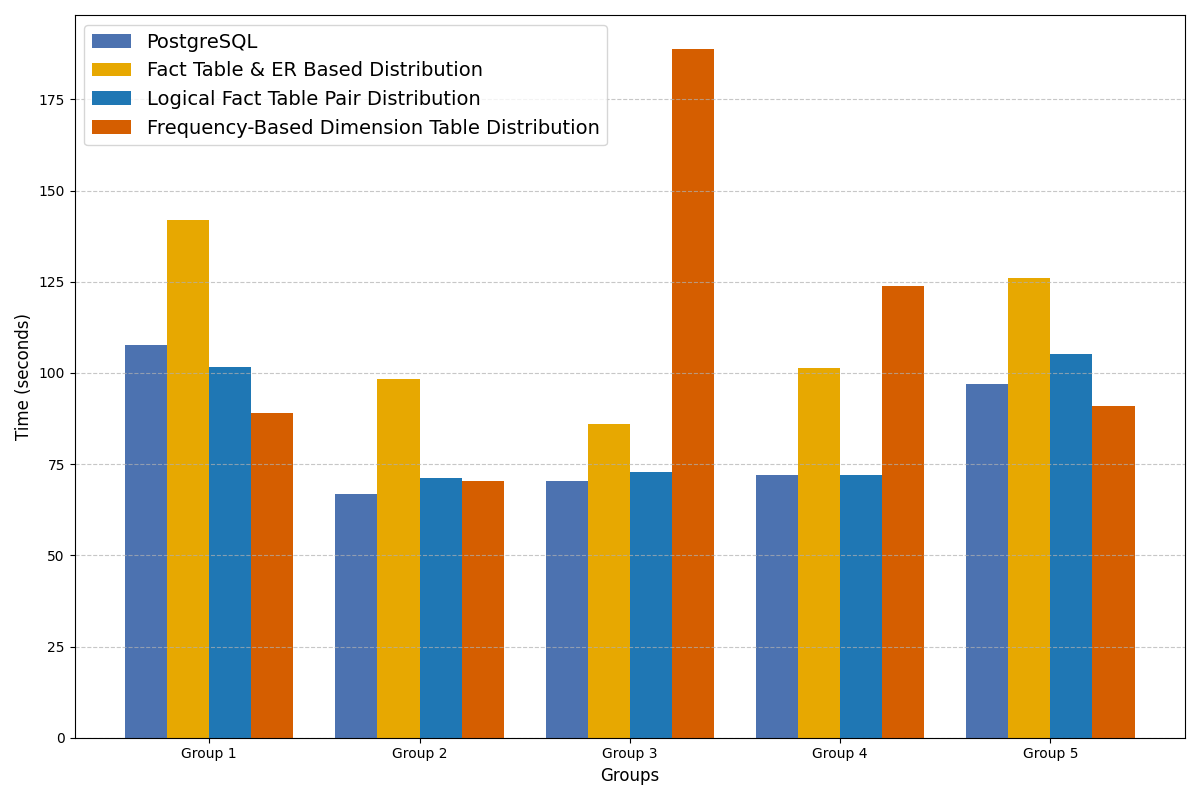
\includegraphics[width=\linewidth]{figures/dist_method_3.png}
    \caption{Average Execution Time by Group - Frequency-Based Dimension Table Distribution}
    \label{fig:dist_method_3}
\end{figure}

Figure~\ref{fig:dist_method_3}  shows the results of the execution with this specific distribution. We observe that in some query groups, the results were not significantly better, with only a small improvement. In other groups, performance was much worse than in the previous strategy, where dimension tables were replicated. For instance, in group 3, we notice a decline in performance by up to 159\%. This outcome can be attributed to the new strategy's reliance on less powerful DBMSs for certain dimension table lookups. When a weaker DBMS, such as Cassandra, handles a dimension table, and its data is then required by a more powerful system for a join, a bottleneck is created. This is because the initial computation and the subsequent data transfer over the network introduce significant overhead, and the entire process now takes longer.



\subsection{Relationship-Aware Dimension Table Distribution}\label{subsec:relationship_dimensions}

To fix the bottleneck of the previous distribution strategy, we implemented a new one. This strategy maintained the principle of not replicating dimension tables in every DBMS, while simultaneously aiming for improved performance. Combined with the frequency of dimension tables’ use in our query workload, we added a second criterion to our approach: their logical relationship to specific fact tables. Dimension tables that are used by all fact tables and appear frequently in queries remained in PostgreSQL, leveraging its superior performance. In contrast, dimension tables that have a logical one-to-one relationship with specific fact tables were placed in the same DBMS as them to avoid redundant data transfer overhead. For instance, the web\_site and web\_page dimension tables, which are used exclusively by web\_sales and web\_returns fact tables, were moved to MongoDB to be physically stored alongside them. All this was done as part of a broader effort to put the dimension tables on our more powerful DBMSs, PostgreSQL and MongoDB. We limited as much as possible those that remained in Cassandra, since our previous results showed that their positioning there hurt the overall performance.
The exact distribution selected in this experiment is shown in Table~\ref{tab:table_distribution_4}.
\begin{table}[htbp]
    \centering
    \renewcommand{\arraystretch}{1.2}
    \caption{Relationship-Aware Dimension Table Distribution Method - Data Distribution}
    \resizebox{\linewidth}{!}{%
        \begin{tabular}{|c|c|c|c|}
            \hline
            Table                   & PostgreSQL & MongoDB    & Cassandra  \\
            \hline
            call\_center            & \          & \          & \checkmark \\
            catalog\_page           & \          & \          & \checkmark \\
            catalog\_returns        & \checkmark & \          & \          \\
            catalog\_sales          & \checkmark & \          & \          \\
            customer                & \checkmark & \          & \          \\
            customer\_address       & \checkmark & \          & \          \\
            customer\_demographics  & \checkmark & \          & \          \\
            date\_dim               & \checkmark & \          & \          \\
            household\_demographics & \checkmark & \          & \          \\
            income\_band            & \          & \checkmark & \          \\
            inventory               & \          & \          & \checkmark \\
            item                    & \checkmark & \          & \          \\
            promotion               & \          & \checkmark & \          \\
            reason                  & \          & \          & \checkmark \\
            ship\_mode              & \          & \          & \checkmark \\
            store                   & \checkmark & \          & \          \\
            store\_returns          & \checkmark & \          & \          \\
            store\_sales            & \checkmark & \          & \          \\
            time\_dim               & \          & \          & \checkmark \\
            warehouse               & \          & \checkmark & \          \\
            web\_page               & \          & \checkmark & \          \\
            web\_returns            & \          & \checkmark & \          \\
            web\_sales              & \          & \checkmark & \          \\
            web\_site               & \          & \checkmark & \          \\
            \hline
        \end{tabular}
    }
    \label{tab:table_distribution_4}
\end{table}

Figure~\ref{fig:dist_method_4} shows the results of the execution with this specific distribution. We now observe a significant improvement in system performance for query groups 3 and 4, which had previously demonstrated very poor results. Specifically, these groups now show an impressive performance improvement of 62\% and 43\%, respectively. Across all query groups, this new distribution strategy consistently demonstrates a slight performance advantage over the Logical Fact Table Pair Distribution strategy, where dimension tables were replicated. The performance improvement averages approximately 1.11\%. This outcome, while modest, aligns with our primary goal of designing an efficient distribution strategy that avoids data redundancy and reduces inter-DBMS communication overhead. Therefore, avoiding data replication across systems is a more favorable design, even if the performance metrics are comparable.

\begin{figure}[htbp]
    \centering
    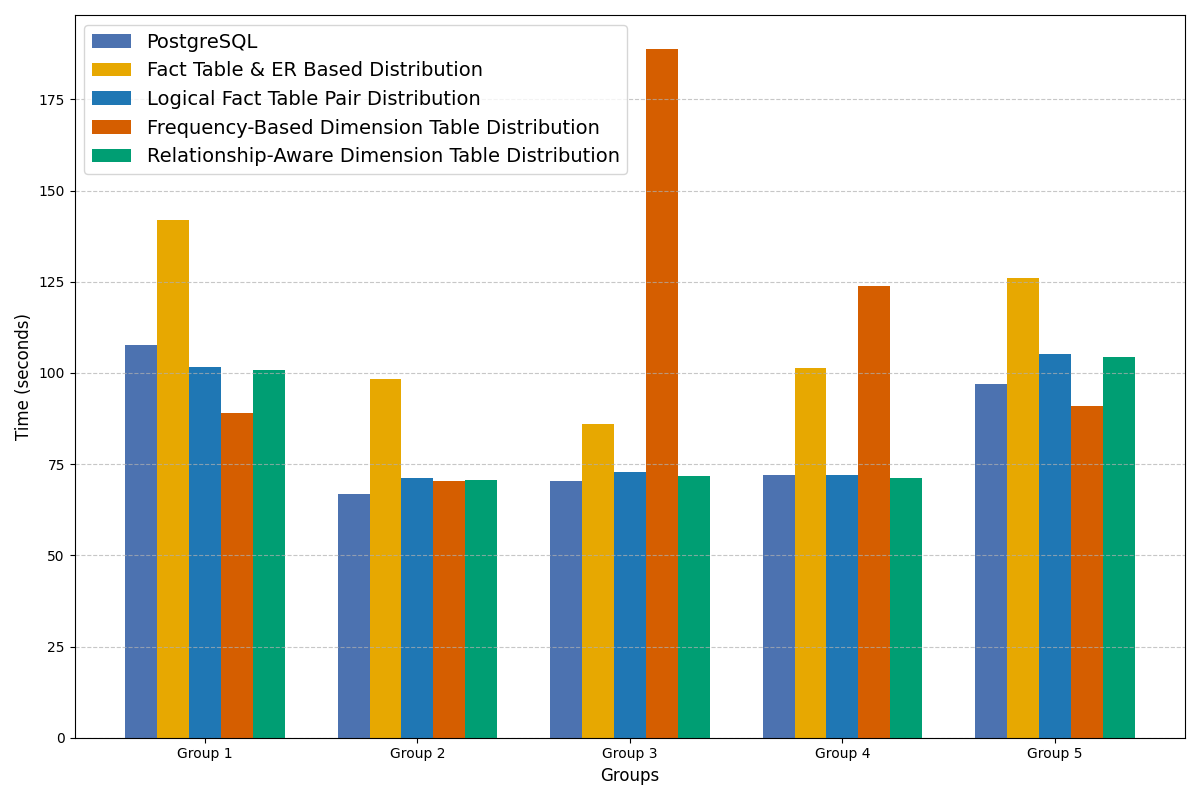
\includegraphics[width=\linewidth]{figures/dist_method_4.png}
    \caption{Average Execution Time by Group - Relationship-Aware Dimension Table Distribution}
    \label{fig:dist_method_4}
\end{figure}


\subsection{Impact of Multi-Worker Execution}

Up to this point, our focus was explicitly centred around different data distribution strategies. We attempted to devise smart plans to allocate data into the three distinct database systems, aiming to optimize query performance. During these experiments, we utilized a single worker node each time. However, PrestoDB provides the opportunity to employ multiple worker nodes working in parallel. In this section, we investigate the impact such configurations have on the distributed query engine’s performance. Specifically, we ran the selected groups of queries using the distribution strategy showcasing the best results – that is, the fourth strategy described in Section~\ref{subsec:relationship_dimensions}, but with the addition of a second, and then, a third working node.
The results of this experiment are shown in Figure~\ref{fig:multiple_workers}.


\begin{figure}[htbp]
    \centering
    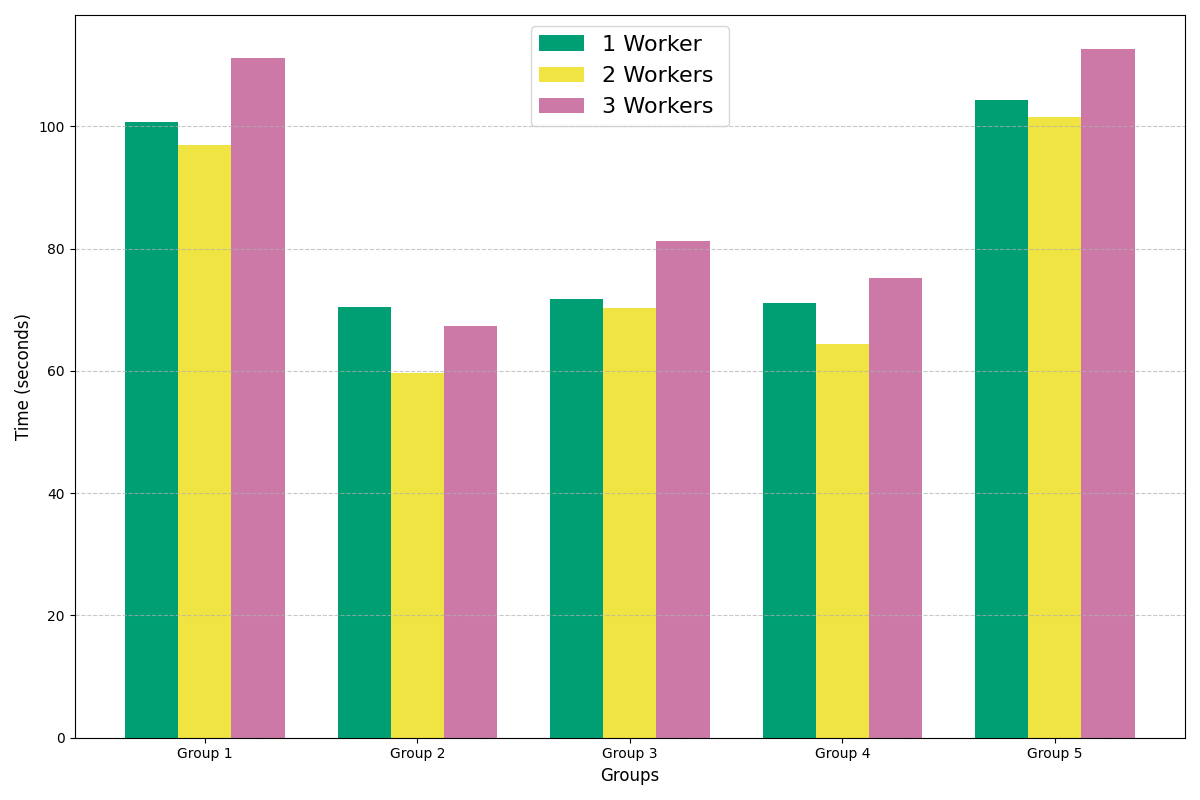
\includegraphics[width=\linewidth]{figures/multiple_workers.png}
    \caption{Average Execution Time by Group - Impact of Multi-Worker Execution}
    \label{fig:multiple_workers}
\end{figure}

The introduction of the second worker led to a general performance improvement, as expected. The improvement was observed across all five complexity groups, with the mean execution time reduction starting from 2.24\% and reaching up to 15.5\%.

The same, however, was not documented with the employment of the third worker. The additional node introduced a significant amount of overhead that not only increased the average query runtime relative to the two-worker setup, but also relative to the single worker. In fact, for query group 3, performance with three workers was 13.1\% worse than with just one. The underlying causes for this discrepancy could vary. For example, a phenomenon that, in all likelihood, contributed heavily to the impaired efficiency is the network and shuffle overhead. Queries, more often than not, require heavy data exchange between workers. As the number of workers increases, the collaboration and communication with one another, understandably, becomes more difficult, potentially leading to the introduced latencies outweighing the benefits. On the other hand, the causation could possibly lie in the small volume of data. For continuity purposes, throughout our experimentations, we kept the amount of generated TPC-DS data constant at 8 GB. However, if the dataset per worker is too small, the overhead of splitting and coordinating tasks may, once again, outweigh the parallelism benefits. Furthermore, we have to also take into consideration the way PrestoDB distributes the different tasks to the workers. Both our worker nodes and database management systems are scattered across two different virtual machines. If the coordinator does not take into account data locality when allocating tasks, the cost of data exchange is sub-optimal. Other potential reasons have also been hypothesized, like the coordinator becoming the bottleneck due to CPU or memory limitations, but through careful monitoring of the available resources, we rejected this idea. Eventually, the truth may lie in any of the aforementioned reasons, or, likely, in a combination of them. Further experimentation is required to pinpoint the exact causes and the extent to which they contribute to the overhead created by the introduction of extra worker nodes.


\section{Conclusion}
To conclude, in this paper, we investigated how the performance of PrestoDB’s distributed execution engine is affected by the operation of queries of varying complexity across different database management systems. More specifically, we measured and compared the execution times registered by PrestoDB on a sufficiently representative subset of TPC-DS benchmarks using different cluster resources and numerous distribution strategies issuing generated data to PostgreSQL, MongoDB, and Apache Cassandra.

Our experiments gave us significant insights into the strengths and weaknesses of each individual DBMS, the effects of data distribution, and the impact of employing multiple workers coordinating in parallel. In brief, we established that PostgreSQL achieves the highest performance across all tested query complexity groups. MongoDB also appears relatively stable in matters of efficiency, while Cassandra becomes less reliable the more query complexity rises. Regarding the different data distribution strategies implemented, none of them managed to outperform the direct runs on PostgreSQL. However, we showcased that through better examination and clever partition, we can approach them very closely. This is of the utmost significance, especially when considering that, in many real-world applications, the allocation of datasets originating from distinct sources is the only realistic option. Lastly, we noted that the increase in the number of workers did not necessarily result in a decrease in total runtime, as hypothesized. Although the introduction of a second worker slightly improved the overall performance, the employment of the third one created, in most cases, a significant amount of overhead, with various possible causes being proposed.

While the aforementioned results provide a solid foundation for understanding the distributed execution engine’s behavior, further research is required to explore unresolved questions and extend our findings. Although the data distribution strategies we devised did not manage to surpass the performance of PostgreSQL, they are by no means the only ones. Further examination could potentially lead to conceiving strategies superior in terms of efficiency. Moreover, supplementary experiments are needed for pinpointing the exact causation of the overhead created by introducing extra workers. Altogether, these directions highlight the need for continued investigation, with the ultimate goal of advancing more efficient and robust distributed systems.

% \bibliographystyle{IEEEtran}
% \bibliography{references}  % no .bib extension


\begin{thebibliography}{00}
    \bibitem{b1} A. Badman and M. Kosinski, ``What is big data?,'' IBM, Nov. 18, 2024. \url{https://www.ibm.com/think/topics/big-data}
    \bibitem{b2} Google Cloud, ``What Is Big Data?'' Google Cloud, 2023. \url{https://cloud.google.com/learn/what-is-big-data}
    \bibitem{b3} ``Overview - Presto 0.294 Documentation,'' Prestodb.io, 2025. \href{https://prestodb.io/docs/current/overview.html}{https://prestodb.io/docs/current/overview.html}.
    \bibitem{b4} R. Sethi et al., ``Presto: SQL on Everything,''
    2019 IEEE 35th International Conference on Data Engineering (ICDE), Apr. 2019.
    \url{https://doi.org/10.1109/icde.2019.00196}.
    \bibitem{b5} ``TPC BENCHMARK\texttrademark DS Standard Specification Version 4.0.0,''
    Transaction Processing Performance Council (TPC), 2024. [Online]. Available: \url{https://www.tpc.org/TPC_Documents_Current_Versions/pdf/TPC-DS_v4.0.0.pdf}
    \bibitem{b6} ``okeanos-knossos IAAS,'' Grnet.gr, 2019.
    \url{https://okeanos-knossos.grnet.gr/}.
    \bibitem{b7} Angelica Lo Duca, T. Meehan, Vivek Bharathan, and Y. Su, Learning and Operating Presto.``O’Reilly Media, Inc.,'' 2023.
    \bibitem{b8} A. Makris, K. Tserpes, G. Spiliopoulos, D. Zissis, and D. Anagnostopoulos, ``MongoDB Vs PostgreSQL: A comparative study on performance aspects,'' \textit{GeoInformatica}, vol. 25, Jun. 2020. doi: \url{https://doi.org/10.1007/s10707-020-00407-w}.

    \bibitem{b9} S. V. Salunke and A. Ouda, ``A Performance Benchmark for the PostgreSQL and MySQL Databases,'' \textit{Future Internet}, vol. 16, no. 10, pp. 382--382, Oct. 2024. doi: \url{https://doi.org/10.3390/fi16100382}.

    \bibitem{b10} S. Juba and A. Volkov, Learning PostgreSQL 11: a beginner’s guide to building high-performance PostgreSQL database solutions, Birmingham, UK: Packt Publishing, 2019.

    \bibitem{b11} S. Yu, ``ACID Properties in Distributed Databases'' Available: \url{https://www.cs.helsinki.fi/group/cinco/teaching/2009/advanced-businesstransactions-seminar/papers/ACID_in_Distributed_Database_Shiwei_Yu.pdf}

    \bibitem{b12} U. Cubukcu, O. A. Erdogan, S. Pathak, S. Sannakkayala, and M. Slot, ``Citus: Distributed PostgreSQL for Data-Intensive Applications,'' in \textit{International Conference on Management of Data}, Jun. 2021. doi: \url{https://doi.org/10.1145/3448016.3457551}.

    \bibitem{b13} PostGIS Developers, ``PostGIS — Spatial and Geographic Objects for PostgreSQL,'' Postgis.net, 2020. \url{https://postgis.net/}.

    \bibitem{b14} V. Abramova and J. Bernardino, ``NoSQL Databases: MongoDB vs Cassandra,'' in \textit{Proceedings of the International C* Conference on Computer Science and Software Engineering - C3S2E ’13}, 2013. doi: \url{https://doi.org/10.1145/2494444.2494447}.

    \bibitem{b15} A. Chauhan, ``A Review on Various Aspects of MongoDb Databases,'' \textit{International Journal of Engineering Research \& Technology}, vol. 8, no. 5, May 2019. \url{https://www.ijert.org/a-review-on-various-aspects-of-mongodb-databases}.

    \bibitem{b16} E. A. Brewer, ``Towards robust distributed systems,'' in \textit{Proceedings of the nineteenth annual ACM symposium on Principles of distributed computing - PODC ’00}, 2000. doi: \url{https://doi.org/10.1145/343477.343502}.

    \bibitem{b17} S. Gilbert and N. Lynch, ``Brewer’s conjecture and the feasibility of consistent, available, partition-tolerant web services,'' \textit{ACM SIGACT News}, vol. 33, no. 2, p. 51, Jun. 2002. doi: \url{https://doi.org/10.1145/564585.564601}.

    \bibitem{b18} S. Gilbert and N. Lynch, ``Perspectives on the CAP Theorem,'' \textit{Computer}, vol. 45, no. 2, pp. 30--36, Feb. 2012. doi: \url{https://doi.org/10.1109/MC.2011.389}.

    \bibitem{b19} G. Wang and J. Tang, ``The NoSQL Principles and Basic Application of Cassandra Model,'' in 2012 \textit{International Conference on Computer Science and Service System}, Aug. 2012. doi: \url{https://doi.org/10.1109/csss.2012.336}.

    \bibitem{b20} H. Tu, ``Cassandra vs. MongoDB: A Systematic Review of Two NoSQL Data Stores in Their Industry Uses,'' in \textit{2024 IEEE 7th International Conference on Big Data and Artificial Intelligence (BDAI)}, Beijing, China, pp. 81--86, Jul. 2024. doi: \url{https://doi.org/10.1109/bdai62182.2024.10692676}.
    \bibitem{b21} R. O. Nambiar and Meikel Poess, ``The making of TPC-DS,''
    in \textit{Proceedings of the 32nd International Conference on Very Large Data Bases (VLDB)}, Sep. 2006, pp. 1049--1058.
    doi: \url{https://doi.org/10.5555/1182635.1164217}
\end{thebibliography}

\end{document}
